\section{Results and Discussions}

\subsection{Quantum Dots}

\begin{frame}


%Two particle 2D
\begin{figure}
 \begin{center}
 \begin{tabular}{c|lll}
  $\omega$ & $\mathrm{E_{VMC}}$ & $\mathrm{E_{DMC}}$ & $\mathrm{E_{FCI}}$\\
\hline\hline
\multicolumn{4}{c}{} \\
 0.01   & \textbf{0.07}406(5)  & \textbf{0.07383}9(2)  & 0.07383505 \\
 0.1    & \textbf{0.44}130(5)  & \textbf{0.44079}(1)   & 0.44079191 \\
 0.28   & \textbf{1.02}215(5)  & \textbf{1.02164}(1)   & 1.0216441  \\
 0.5    & \textbf{1.6}6021(5)  & \textbf{1.65977}(1)   & 1.6597723  \\
 1.0    & \textbf{3.000}30(5)  & \textbf{3.00000}(1)   & 3.0000001  \\
\cline{1-4}
 \end{tabular}  
 \end{center}
  \caption{Two-particle results for two-dimensional quantum dots compared with FCI results by Veronica K.B. Olsen.}
\end{figure}
\end{frame}


%Two particle 42 56 2D
\begin{frame}

\begin{figure}
 \begin{center}
 \footnotesize
 \begin{tabular}{cc|llll}
 N      &  $\omega$ & $\mathrm{E_{VMC}}$ & $\mathrm{E_{DMC}}$ & $\mathrm{E_{SRG}}$ & $\mathrm{E_{CCSD}}$\\
\hline\hline
\multicolumn{6}{c}{} \\
    42    &   0.1    & 107.881(1)  & 107.6389(2) &- 			& 111.7170 \{8\} \\
          &   0.28   & 220.161(1)  & 219.8426(2) &219.8836 \{14\}	& 222.1401 \{8\} \\
          &   0.5    & 331.002(1)  & 330.6306(2) &330.6485 \{14\}	& 331.8901 \{8\} \\
          &   1.0    & 544.2(8)    & 542.9428(8) &542.9528 \{14\}	& 543.1155 \{18\}\\
\cline{2-6}
\multicolumn{6}{c}{} \\
    56    &   0.1    & 176.269(2) & 175.9553(7)  & -		& 186.1034 \{9\} \\
          &   0.28   & 358.594(2) & 358.145(2)   & -		& 363.2048 \{9\} \\
          &   0.5    & 538.5(6)   & 537.353(2)   & -		& 540.3430 \{9\} \\
          &   1      & 880.2(7)   & 879.3986(6)  & -		& 879.6386 \{17\}\\
\cline{2-6}
 \end{tabular}  
 \end{center}
  \caption{Results for two-dimensional quantum dots 42 and 56 particles compared with SRG results by Sarah Reimann and CCSD results by Christoffer Hirth.}
\end{figure}
\end{frame}

\normalsize

%Two particle 2D
\begin{frame}

\footnotesize
\begin{figure}
 \begin{center}
 \begin{tabular}{cc|rrr}
    N     & $\omega$ & $\mathrm{E_{VMC}}$ & $\mathrm{E_{DMC}}$ & $\mathrm{E_0}$\\
\hline\hline
\multicolumn{5}{c}{} \\
    2     &   0.01   & 0.07939(3)  & 0.079206(3) & -		\\
          &   0.1    & 0.50024(8)  & 0.499997(3) & 0.5        \\
          &   0.28   & 1.20173(5)  & 1.201725(2) & -		\\
          &   0.5    & 2.00005(2)  & 2.000000(2) & 2.0 \\
          &   1.0    & 3.73032(8)  & 3.730123(3) & - \\
% \cline{2-5}
% \multicolumn{5}{c}{} \\
%     8     &   0.1    & 5.7130(6)   & 5.7028(1)   & - 		\\
%           &   0.28   & 12.2040(8)  & 12.1927(1)  & -		\\
%           &   0.5    & 18.9750(7)  & 18.9611(1)  & -\\
%           &   1.0    & 32.6842(8)  & 32.6680(1)  & -\\
% \cline{2-5}
% \multicolumn{5}{c}{} \\
%     20    &   0.1    & 27.316(2)   & 27.2717(2)   & - 		\\
%           &   0.28   & 56.440(2)   & 56.3868(2)   & -		\\
%           &   0.5    & 85.714(2)   & 85.6555(2)   & - \\
%           &   1.0    & 142.951(2)  & 142.8875(2)  & -
 \end{tabular}  
 \end{center}
  \caption{Results for three-dimensional quantum dots compared with exact solutions by M. Taut.}
\end{figure}
\end{frame}

\normalsize


 
 \begin{frame}
  \captionsetup[subfloat]{labelformat=empty}
\begin{figure}
 \begin{center}
  \subfigure[$N=2$]{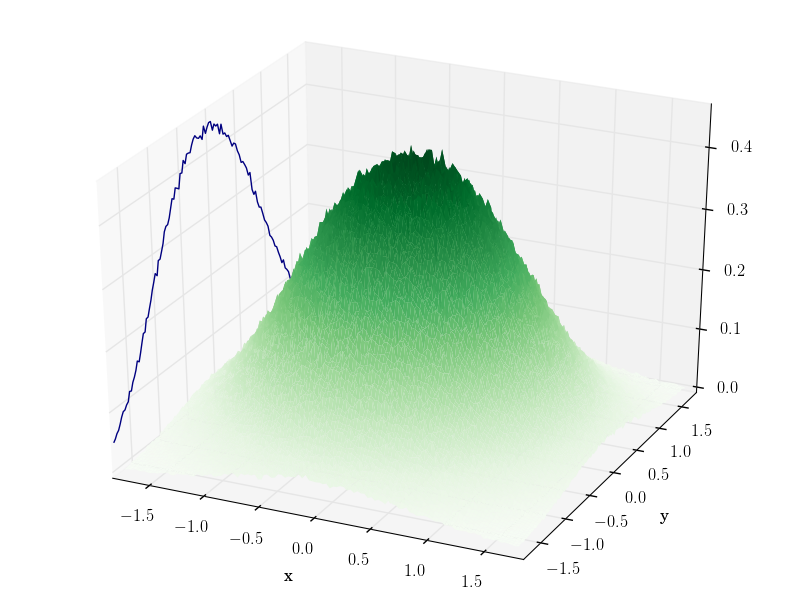
\includegraphics[scale=0.15]{../graphics/OBD/OBD_DMC/dist_out_QDots2c1_3D.png}}
  \subfigure[$N=12$]{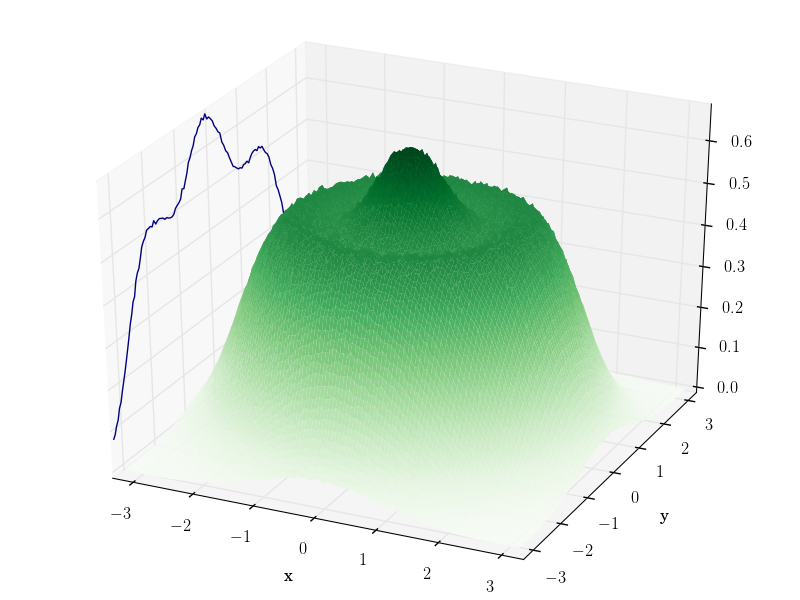
\includegraphics[scale=0.15]{../graphics/OBD/OBD_DMC/dist_out_QDots12c1_3D.png}}
  \subfigure[$N=30$]{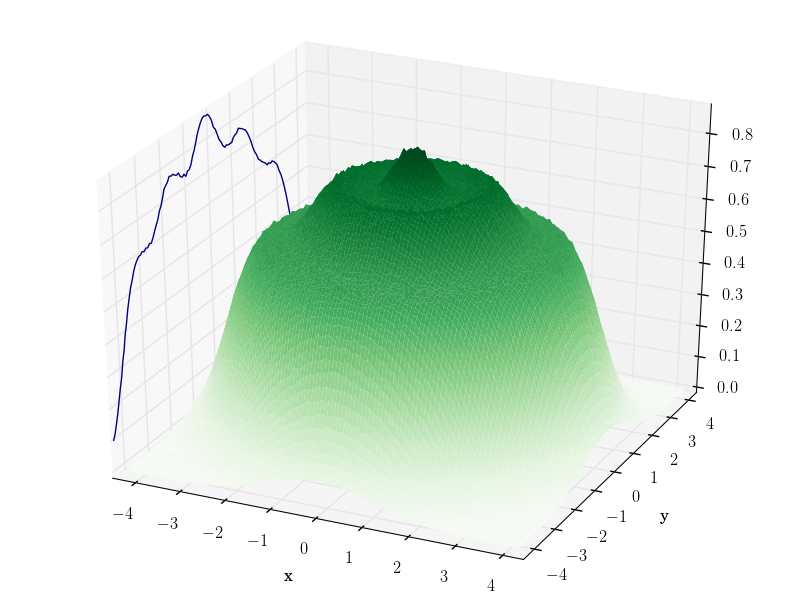
\includegraphics[scale=0.15]{../graphics/OBD/OBD_DMC/dist_out_QDots30c1_3D.png}}\\
  \subfigure[$N=6$]{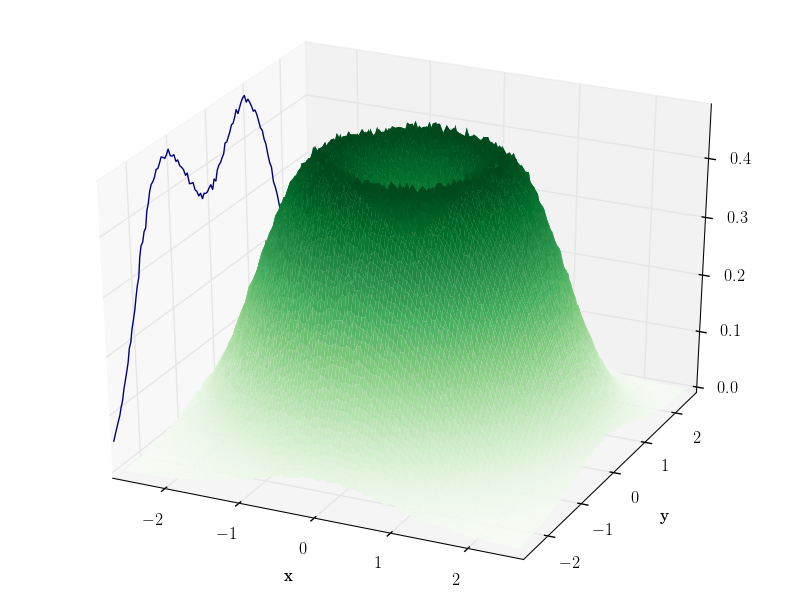
\includegraphics[scale=0.15]{../graphics/OBD/OBD_DMC/dist_out_QDots6c1_3D.png}} 
  \subfigure[$N=20$]{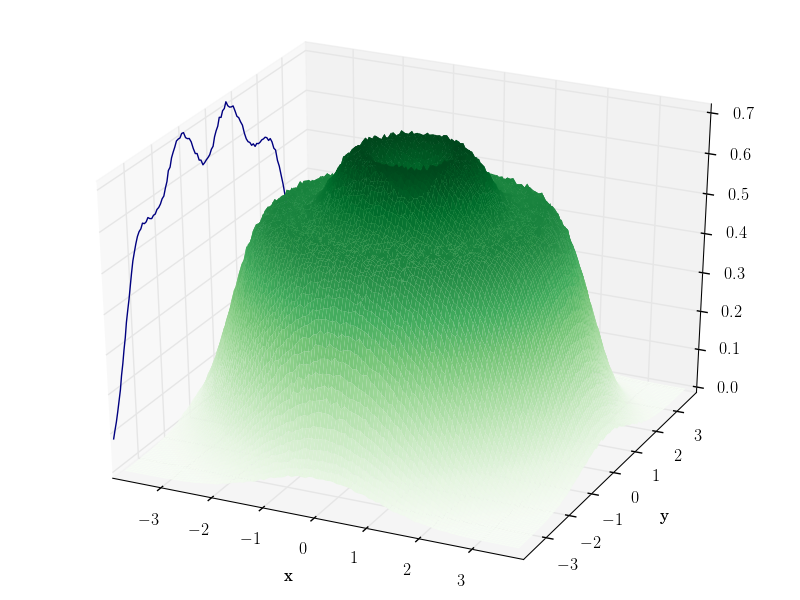
\includegraphics[scale=0.15]{../graphics/OBD/OBD_DMC/dist_out_QDots20c1_3D.png}} 
  \subfigure[$N=42$]{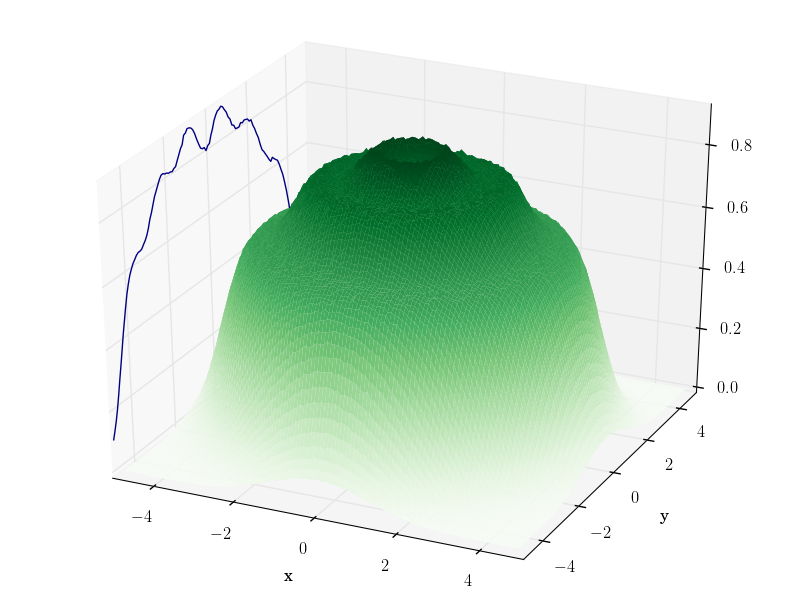
\includegraphics[scale=0.15]{../graphics/OBD/OBD_DMC/dist_out_QDots42c1_3D.png}} \\
  \caption{DMC one-body densities for two-dimensional quantum dots.}
  \label{fig:OBD_DMC_QDOTS_w1} 
 \end{center}
\end{figure}
 \end{frame}

\begin{frame}

% \begin{center}
% \begin{tabular}{cc}
% VMC density & $|\Psi_T(\mathbf{r})|^2$ \\
% &  \\
% DMC density & $\Phi(\mathbf{r}, \tau)\Psi_T(\mathbf{r})$ \\
% &  \\
% Pure density & $|\Phi(\mathbf{r}, \tau)|^2$  
% \end{tabular}
% \end{center}

\end{frame}
 
\begin{frame}

\begin{figure}
 \begin{center}
 \begin{tabular}{cc|c}
   \subfigure{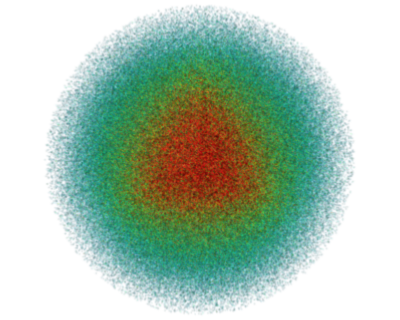
\includegraphics[scale=0.15]{../graphics/OBD/OBD_Q3D/QD2w1_3D.png}} &
   \subfigure{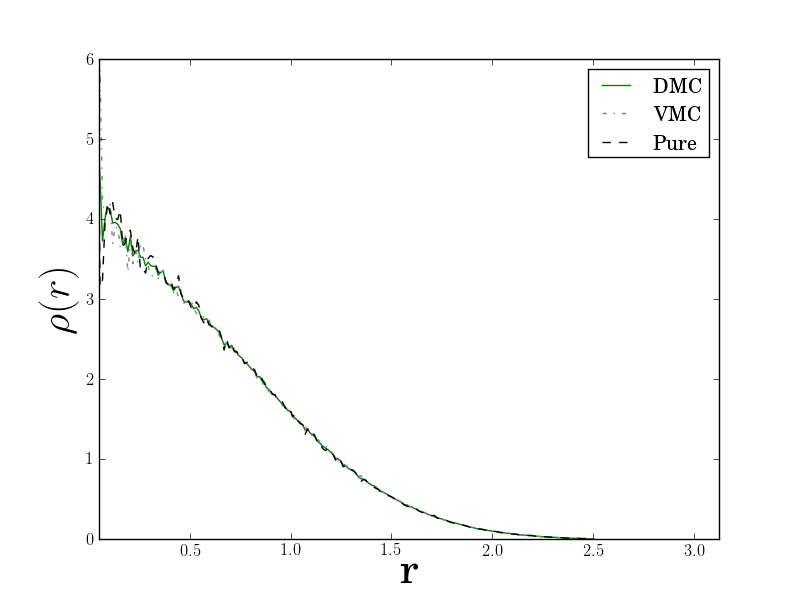
\includegraphics[scale=0.12]{../graphics/OBD/OBD_Q3D/QD2w1_2D.png}} &
   \subfigure{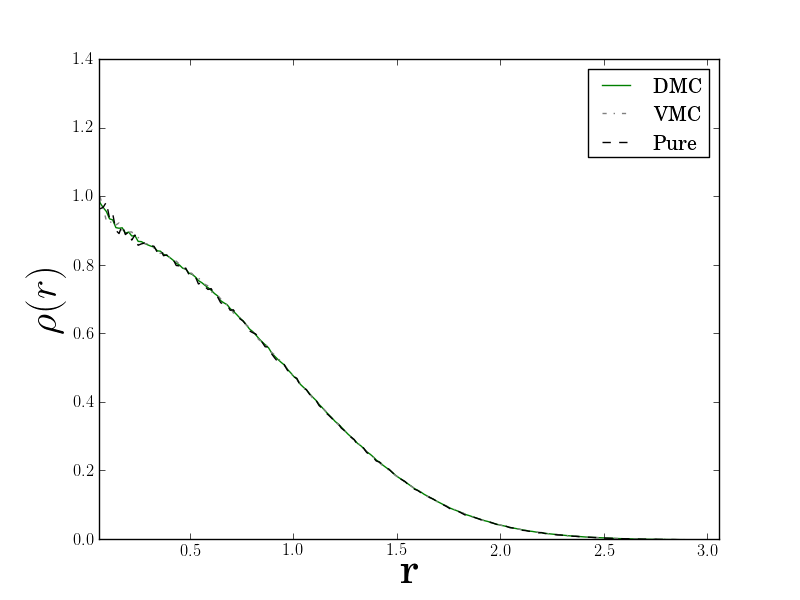
\includegraphics[scale=0.12]{../graphics/OBD/OBD_Q3D/comp/Q2D_2.png}} \\
   \subfigure{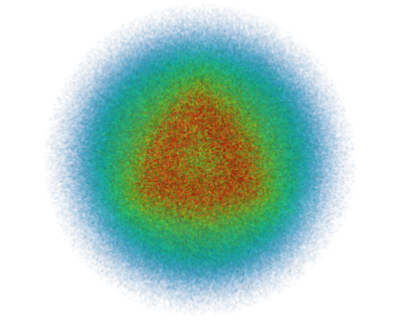
\includegraphics[scale=0.15]{../graphics/OBD/OBD_Q3D/QD8w1_3D.png}} &
   \subfigure{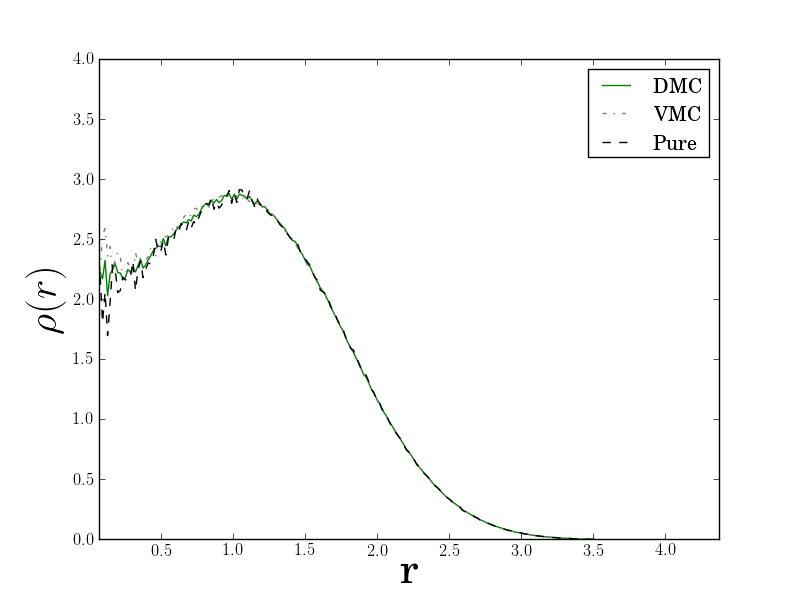
\includegraphics[scale=0.12]{../graphics/OBD/OBD_Q3D/QD8w1_2D.png}} & 
   \subfigure{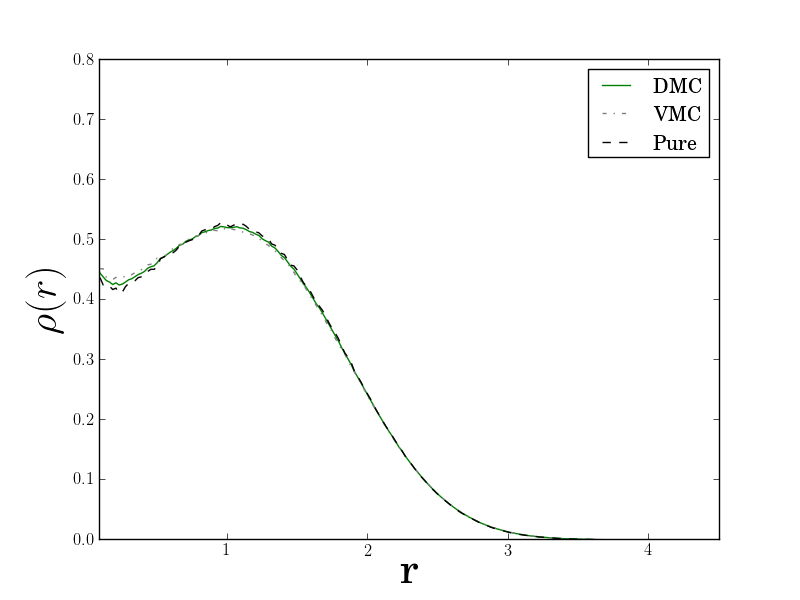
\includegraphics[scale=0.12]{../graphics/OBD/OBD_Q3D/comp/Q2D_6.png}} \\
   \subfigure{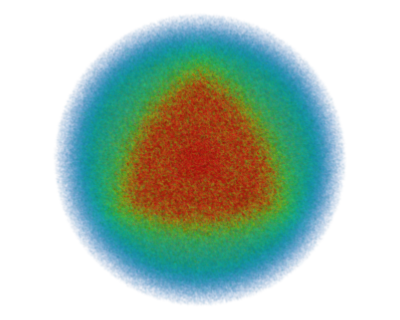
\includegraphics[scale=0.15]{../graphics/OBD/OBD_Q3D/QD20w1_3D.png}} &
   \subfigure{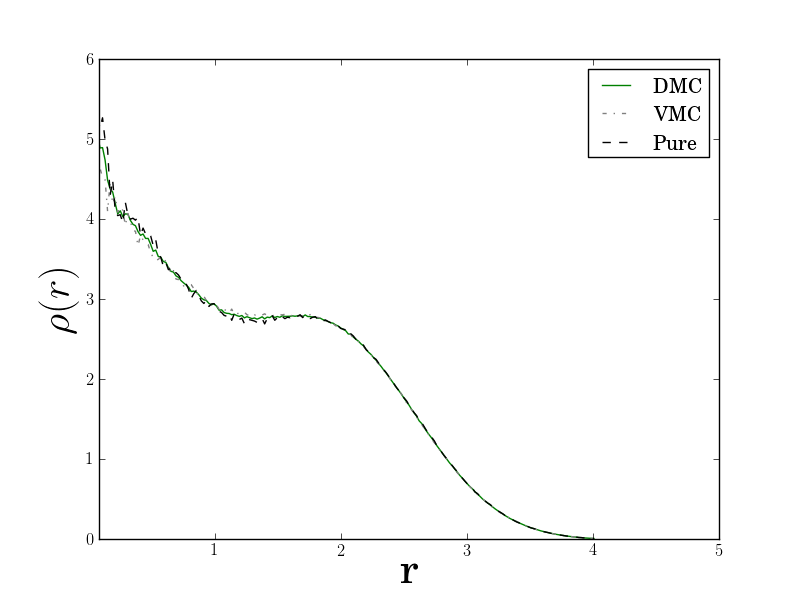
\includegraphics[scale=0.12]{../graphics/OBD/OBD_Q3D/QD20w1_2D.png}} & 
   \subfigure{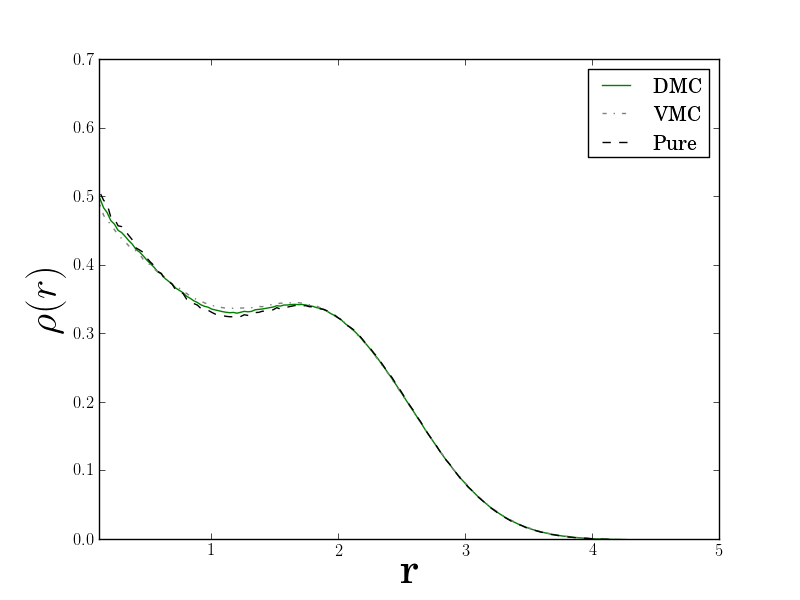
\includegraphics[scale=0.12]{../graphics/OBD/OBD_Q3D/comp/Q2D_12.png}} \\
  \end{tabular}
  \caption{One-body densities for two- and three-dimensional quantum dots.}
  \label{fig:OBD_QDOTS3D_highfreq}
 \end{center}
\end{figure}

\end{frame}


\begin{frame}
\frametitle{Lowering the frequency}

\setlength{\tabcolsep}{0.1pt}
\def\arraystretch{0}
\begin{figure}
 \begin{center}
 \begin{tabular}{rl}
   \footnotesize{\rot{$\qquad\omega=1$}}&\subfigure{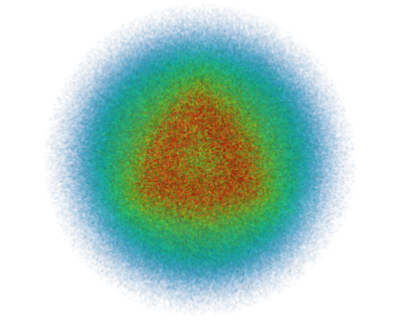
\includegraphics[scale=0.2]{../graphics/OBD/OBD_Q3D/QD8w1_3D.png}}
   \subfigure{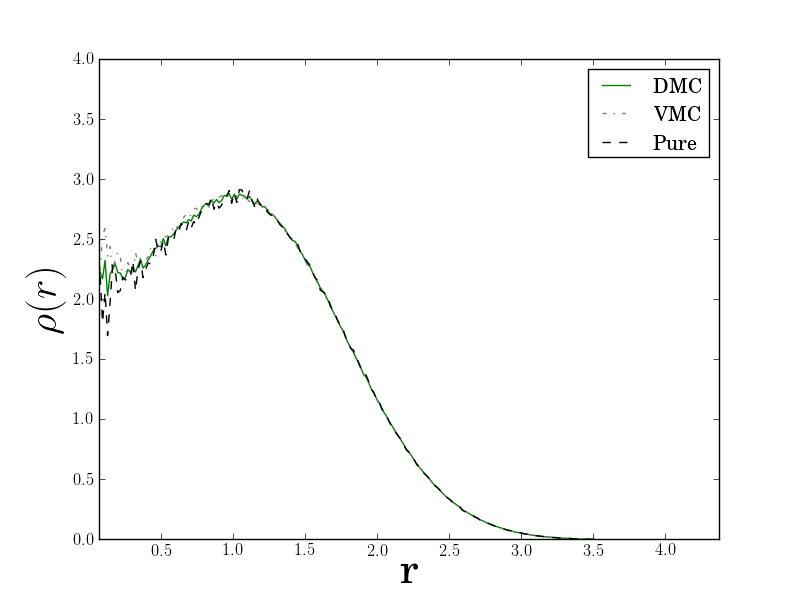
\includegraphics[scale=0.17]{../graphics/OBD/OBD_Q3D/QD8w1_2D.png}} \\
   \footnotesize{\rot{$\quad\,\,\omega=0.01$}}&\subfigure{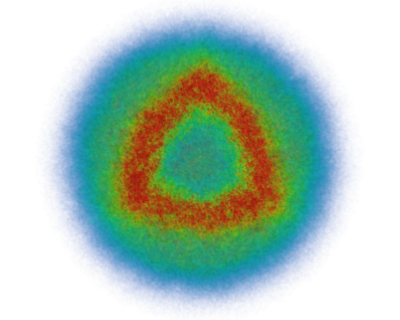
\includegraphics[scale=0.2]{../graphics/OBD/OBD_Q3D/QD8w001_3D.png}} 
   \subfigure{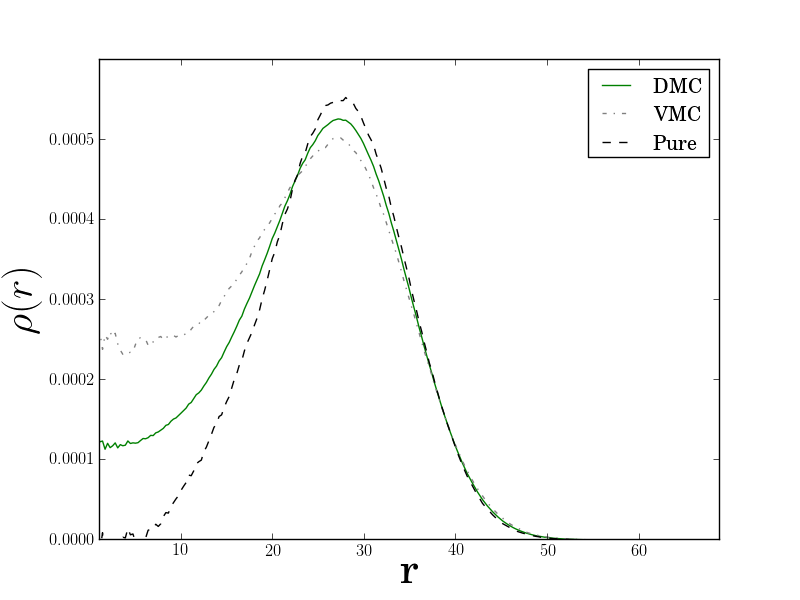
\includegraphics[scale=0.17]{../graphics/OBD/OBD_Q3D/QD8w001_2D.png}} 
  \end{tabular}
  \caption{One-body densities for a 8-particle three-dimensional quantum dot for high and low frequencies.}
  \label{fig:OBD_QDOTS3D_lowfreq}
 \end{center}
\end{figure}
\def\arraystretch{1}
\end{frame}


\begin{frame}

\captionsetup[subfloat]{labelformat=empty}

\tiny
\begin{figure}
 \begin{center}
 \begin{tabular}{rl}
  \rot{$\qquad\omega=0.28$}&\subfigure{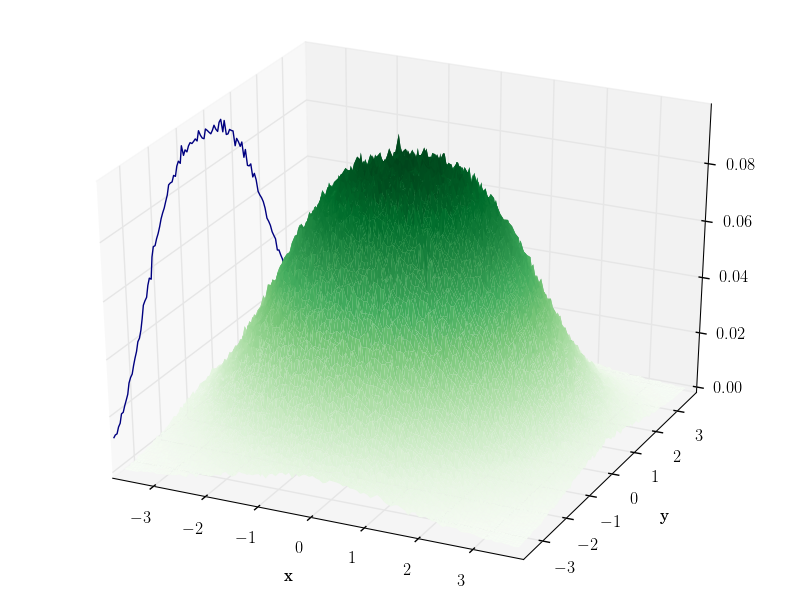
\includegraphics[scale=\OBDscale]{../graphics/OBD/OBD_DMC/dist_out_QDots2c028_3D.png}}
  \subfigure{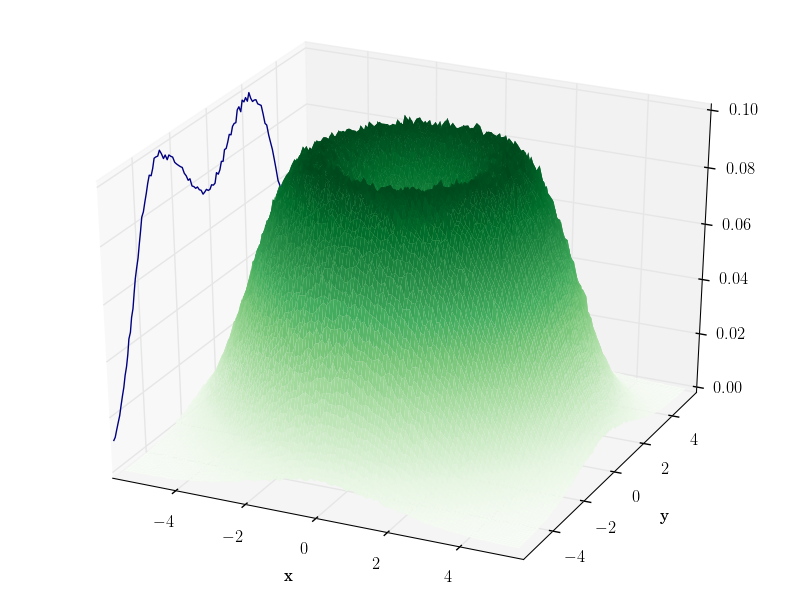
\includegraphics[scale=\OBDscale]{../graphics/OBD/OBD_DMC/dist_out_QDots6c028_3D.png}} 
  \subfigure{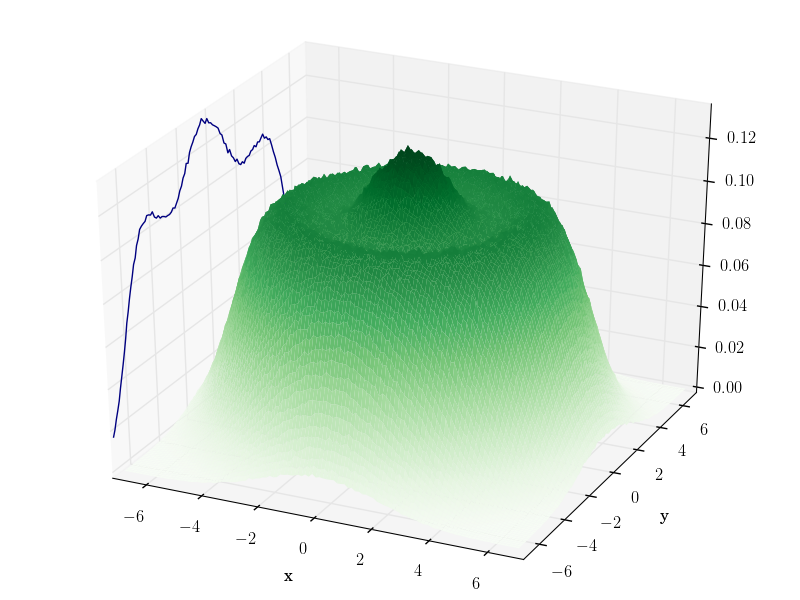
\includegraphics[scale=\OBDscale]{../graphics/OBD/OBD_DMC/dist_out_QDots12c028_3D.png}}
  \subfigure{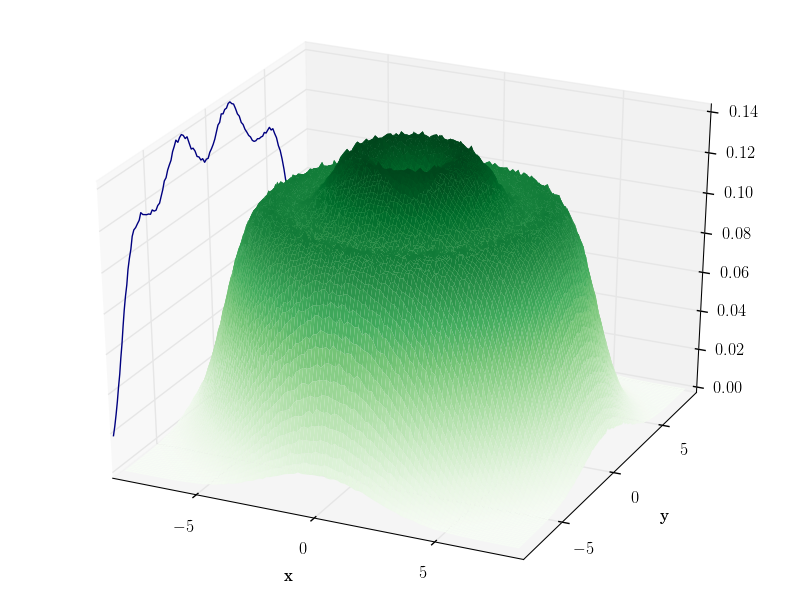
\includegraphics[scale=\OBDscale]{../graphics/OBD/OBD_DMC/dist_out_QDots20c028_3D.png}} \\[-0pt]
  \rot{$\qquad\omega=0.1$}&\subfigure{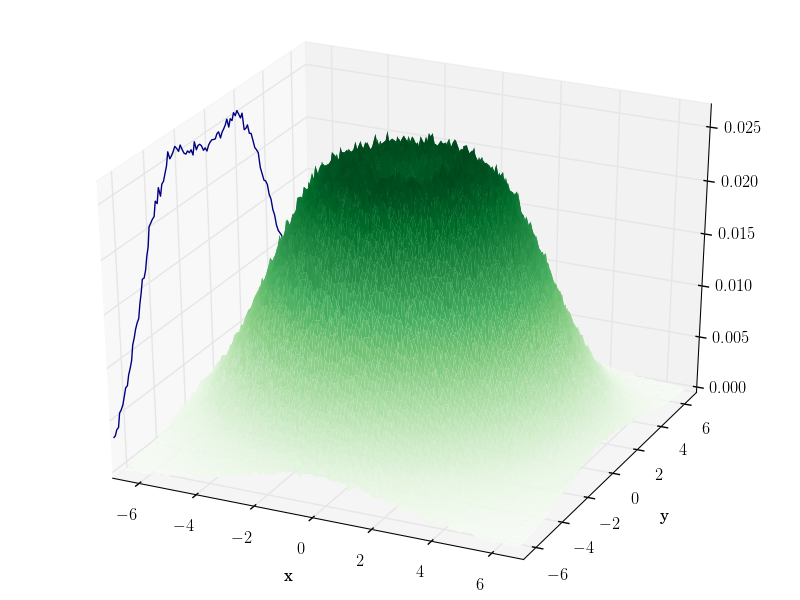
\includegraphics[scale=\OBDscale]{../graphics/OBD/OBD_DMC/dist_out_QDots2c01_3D.png}}
  \subfigure{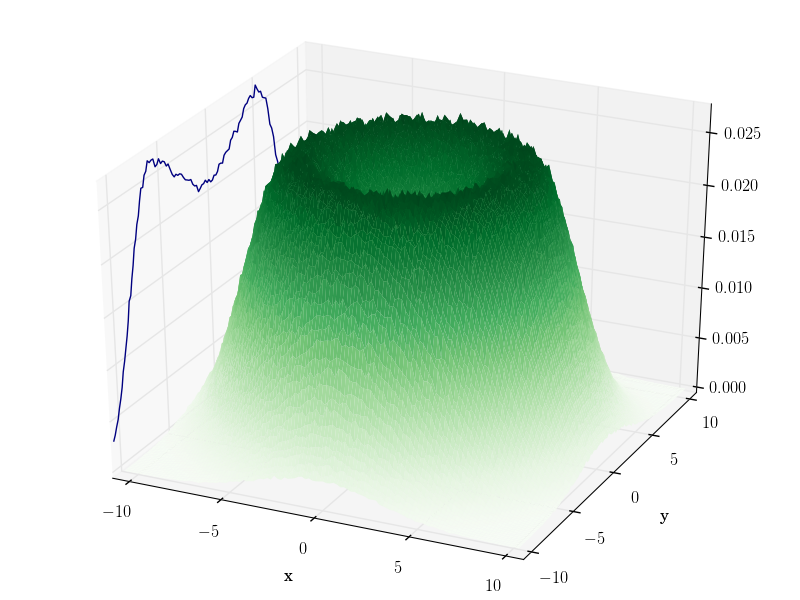
\includegraphics[scale=\OBDscale]{../graphics/OBD/OBD_DMC/dist_out_QDots6c01_3D.png}} 
  \subfigure{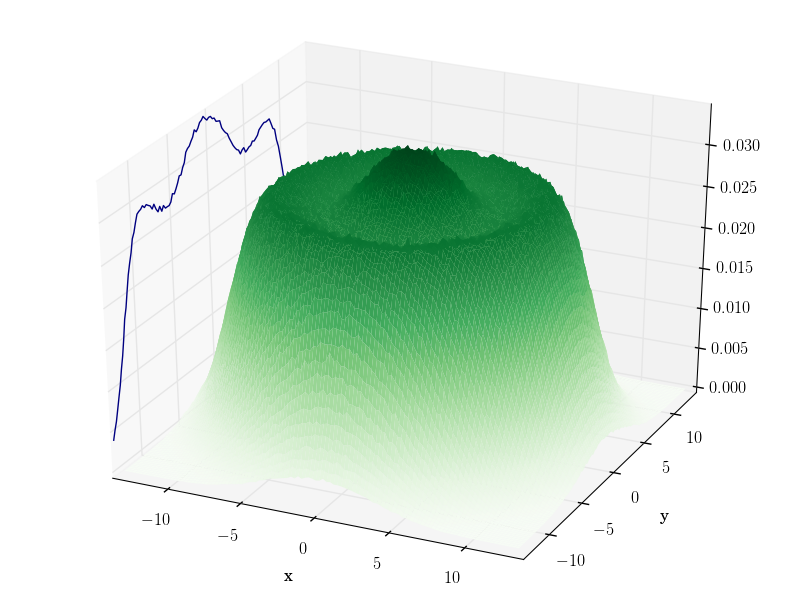
\includegraphics[scale=\OBDscale]{../graphics/OBD/OBD_DMC/dist_out_QDots12c01_3D.png}}
  \subfigure{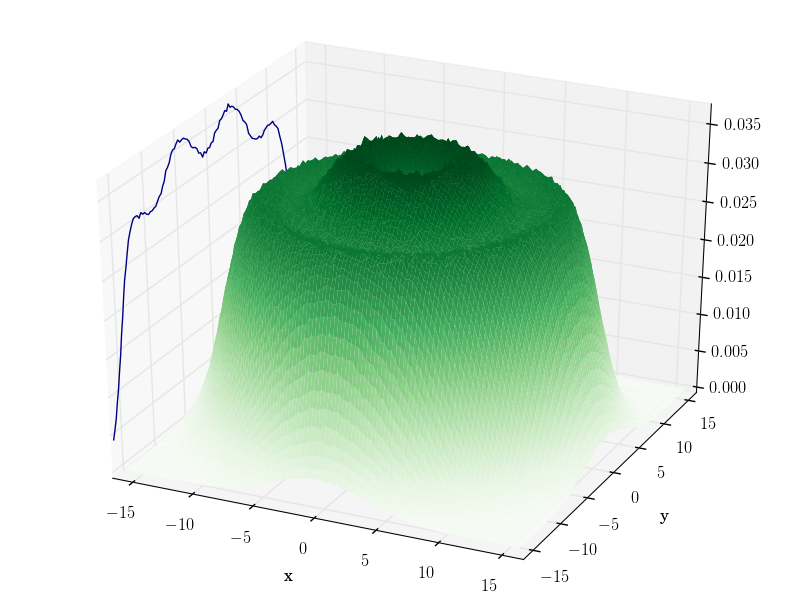
\includegraphics[scale=\OBDscale]{../graphics/OBD/OBD_DMC/dist_out_QDots20c01_3D.png}} \\[-0pt]
  \rot{$\qquad\omega=0.01$}&\subfigure[$N=2$]{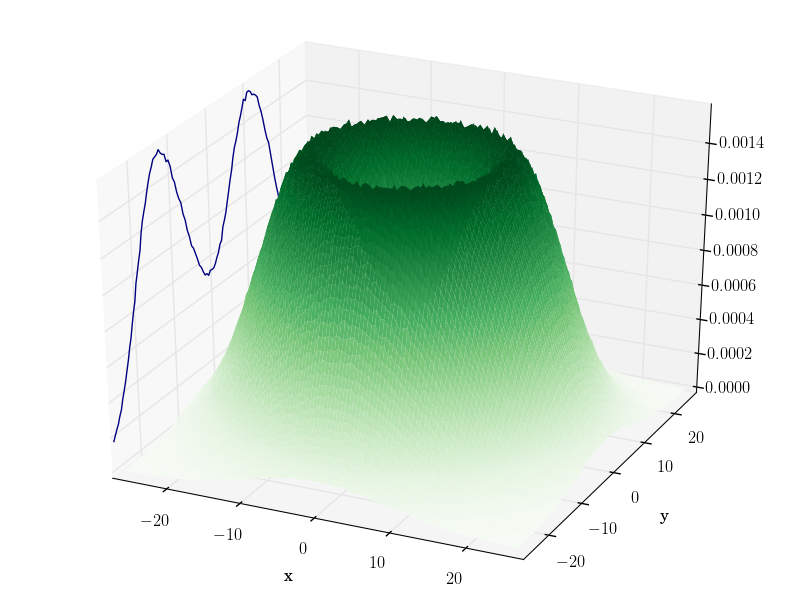
\includegraphics[scale=\OBDscale]{../graphics/OBD/OBD_DMC/dist_out_QDots2c001_3D.png}}
  \subfigure[$N=6$]{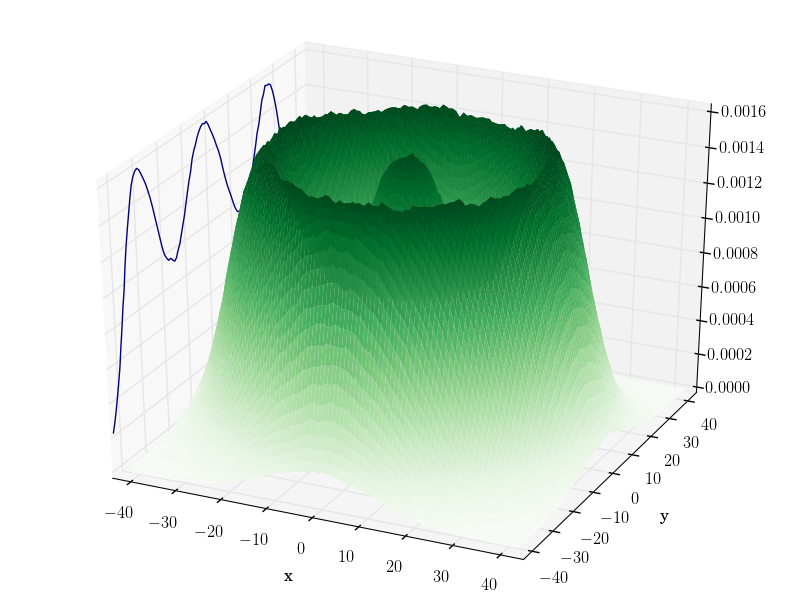
\includegraphics[scale=\OBDscale]{../graphics/OBD/OBD_DMC/dist_out_QDots6c001_3D.png}} 
  \subfigure[$N=12$]{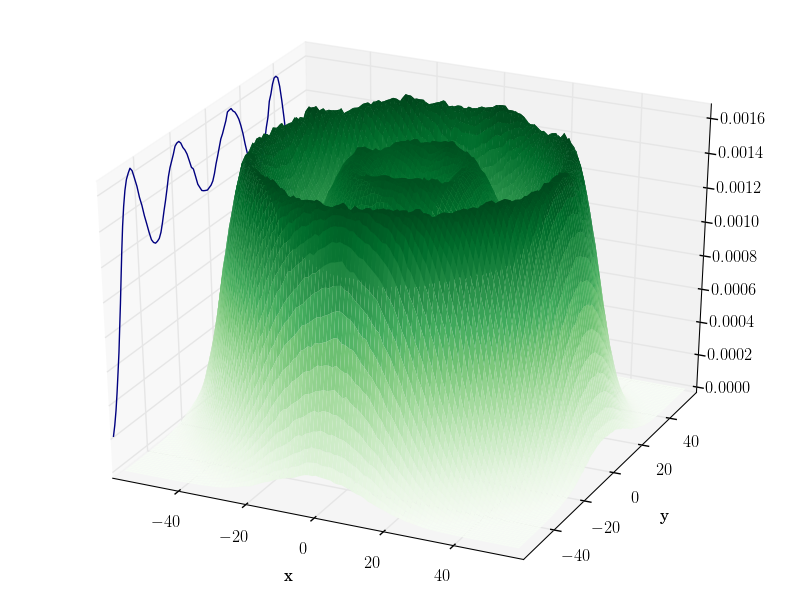
\includegraphics[scale=\OBDscale]{../graphics/OBD/OBD_DMC/dist_out_QDots12c001_3D.png}}
  \subfigure[$N=20$]{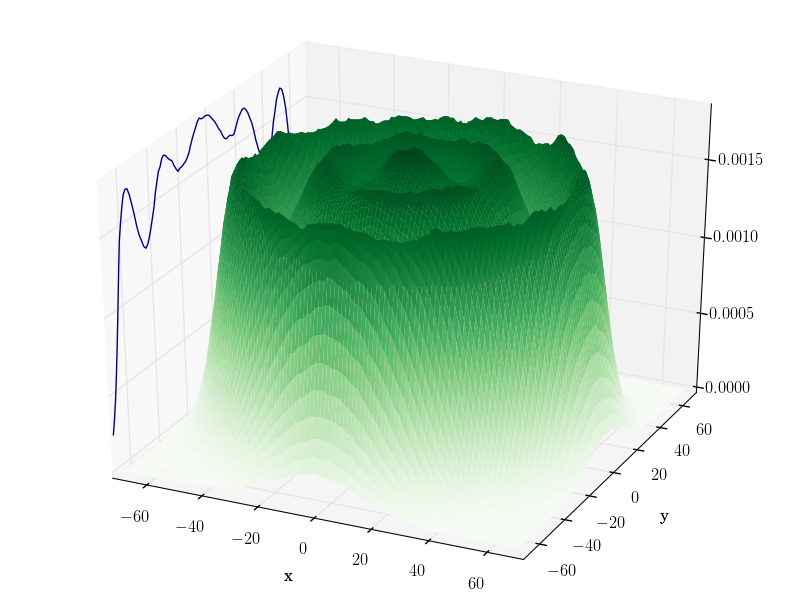
\includegraphics[scale=\OBDscale]{../graphics/OBD/OBD_DMC/dist_out_QDots20c001_3D.png}} \\
 \end{tabular}
  \label{fig:OBD_DMC_QDOTS_lowering3D}
 \end{center}
\end{figure}
\setlength{\tabcolsep}{6pt}
\normalsize

\end{frame}

\begin{frame}
 The electrons become more \textit{localized} and dilute. 
 \shift
 
 The two- and three-dimensional densities no longer match.
 \shift
 
 Transition into a new region? 
\end{frame}


\begin{frame}
\frametitle{Electron crystals for N=6}
 \begin{figure}
 \begin{center}
  \subfigure{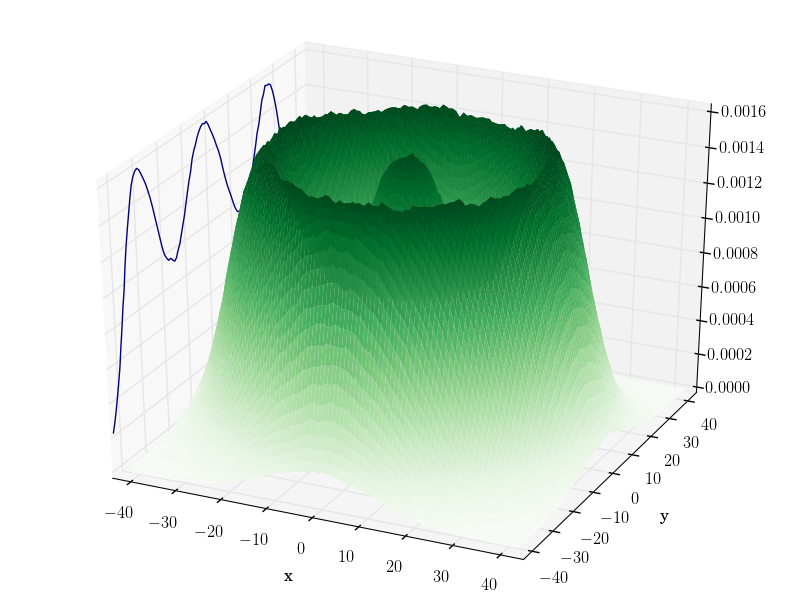
\includegraphics[scale=0.25]{../graphics/OBD/OBD_DMC/dist_out_QDots6c001_3D.png}}
  \subfigure{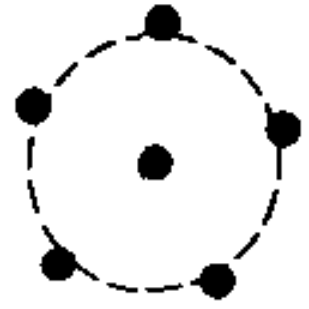
\includegraphics[scale=0.2]{../graphics/wigner/wigner6.png}}
  \label{fig:wigner20}
  \caption{OBD for a 6-particle two-dimensional quantum dot compared to the classical theoretical configuration taken from F. Bolton, U. Rössler.  \textit{Superlattices and microstructures} \textbf{13}, 139 (1993).}
 \end{center}
\end{figure}
\end{frame}

\begin{frame}
\frametitle{Electron crystals for N=6 (frozen)}
 \begin{figure}
 \begin{center}
  \subfigure{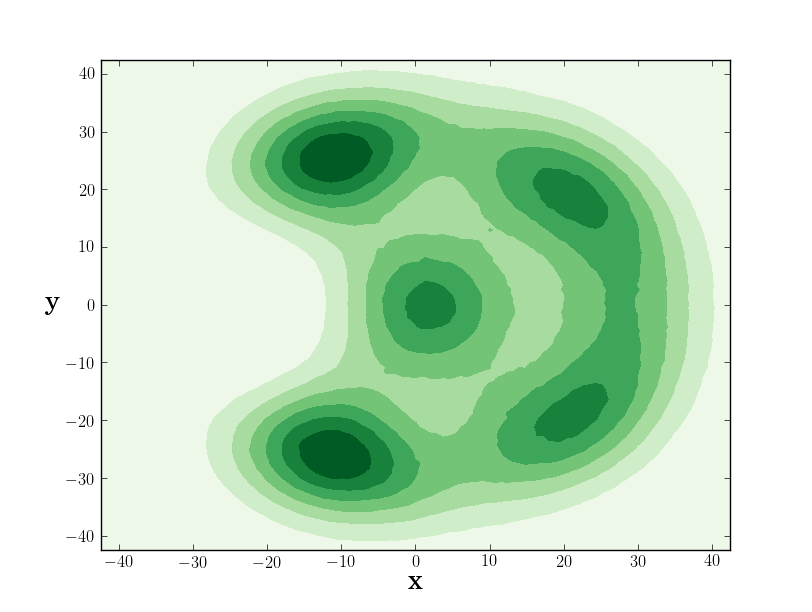
\includegraphics[scale=0.25]{../graphics/wigner/locked6_2d.png}}
  \subfigure{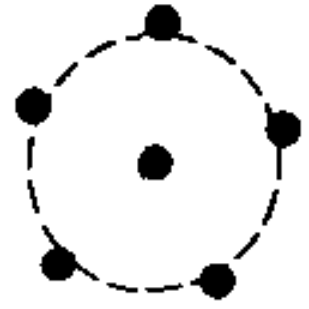
\includegraphics[scale=0.2]{../graphics/wigner/wigner6.png}}
  \label{fig:wigner20}
  \caption{OBD for a 6-particle two-dimensional quantum dot compared to the classical theoretical configuration taken from F. Bolton, U. Rössler.  \textit{Superlattices and microstructures} \textbf{13}, 139 (1993).}
 \end{center}
\end{figure}
\end{frame}

\begin{frame}
\frametitle{Electron crystals for N=6 (frozen)}
 \begin{figure}
 \begin{center}
  \subfigure{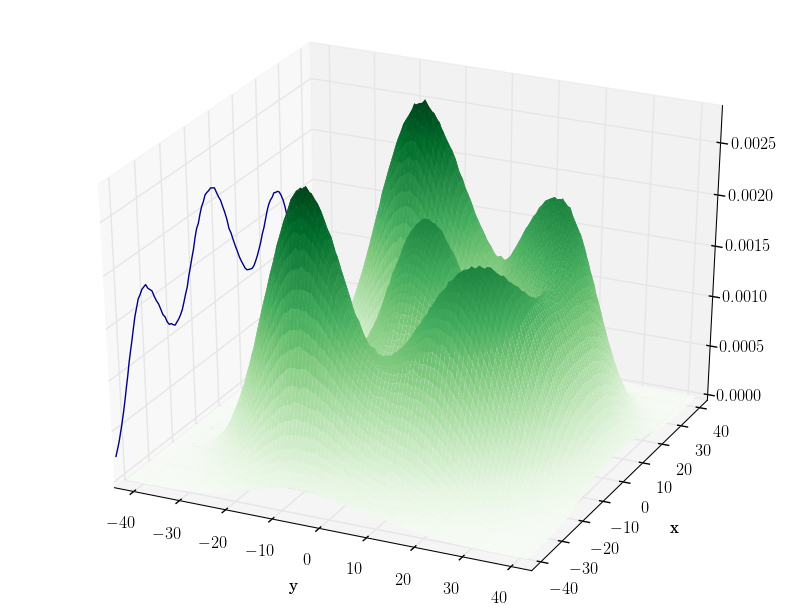
\includegraphics[scale=0.25]{../graphics/wigner/locked6_3d.png}}
  \subfigure{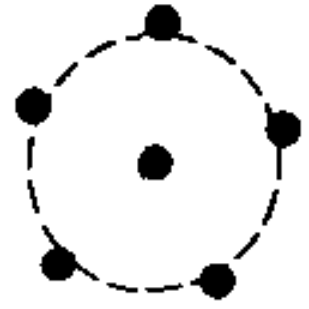
\includegraphics[scale=0.2]{../graphics/wigner/wigner6.png}}
  \label{fig:wigner20}
  \caption{OBD for a 6-particle two-dimensional quantum dot compared to the classical theoretical configuration taken from F. Bolton, U. Rössler.  \textit{Superlattices and microstructures} \textbf{13}, 139 (1993).}
 \end{center}
\end{figure}
\end{frame}

\begin{frame}
\frametitle{Electron crystals for N=12}
 \begin{figure}
 \begin{center}
  \subfigure{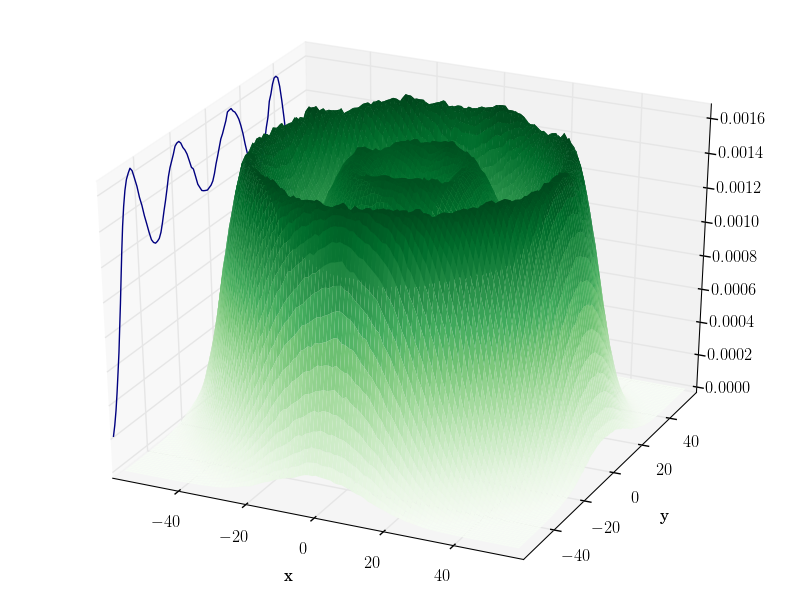
\includegraphics[scale=0.25]{../graphics/OBD/OBD_DMC/dist_out_QDots12c001_3D.png}}
  \subfigure{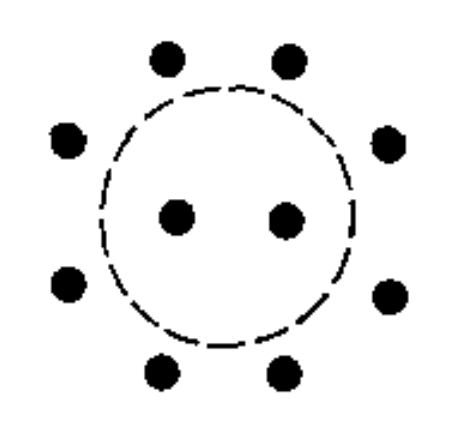
\includegraphics[scale=0.2]{../graphics/wigner/wigner10.png}}
  \label{fig:wigner20}
  \caption{OBD for a 12-particle two-dimensional quantum dot compared to the classical theoretical configuration taken from F. Bolton, U. Rössler.  \textit{Superlattices and microstructures} \textbf{13}, 139 (1993).}
 \end{center}
\end{figure}
\end{frame}

\begin{frame}
\frametitle{Electron crystals for N=12 (frozen)}
 \begin{figure}
 \begin{center}
  \subfigure{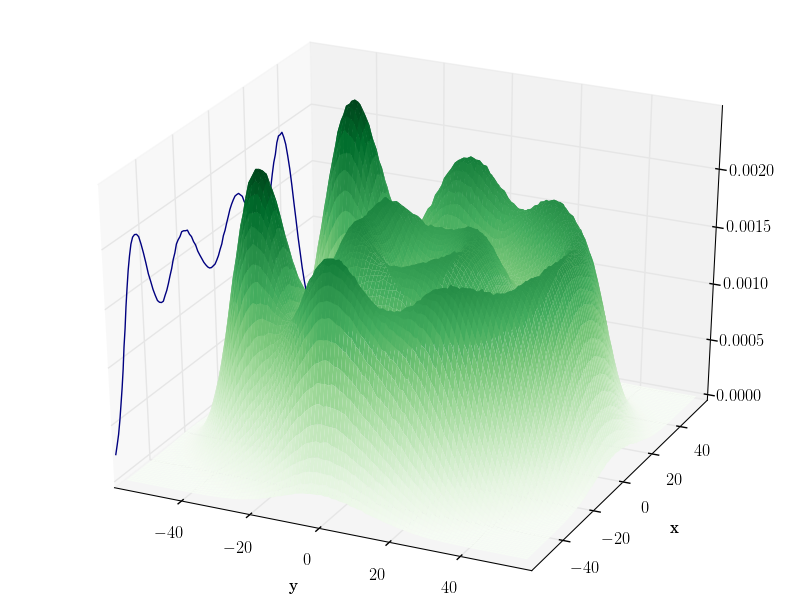
\includegraphics[scale=0.25]{../graphics/wigner/locked12_3d.png}}
  \subfigure{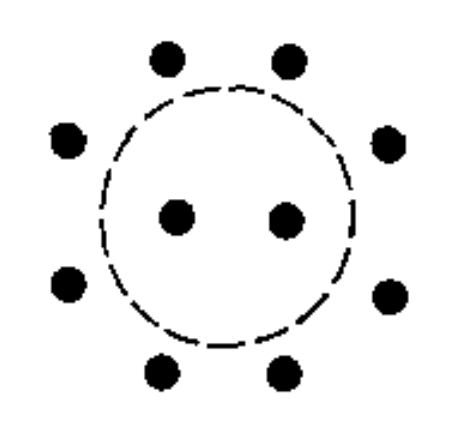
\includegraphics[scale=0.2]{../graphics/wigner/wigner10.png}}
  \label{fig:wigner20}
  \caption{OBD for a 12-particle two-dimensional quantum dot compared to the classical theoretical configuration taken from F. Bolton, U. Rössler.  \textit{Superlattices and microstructures} \textbf{13}, 139 (1993).}
 \end{center}
\end{figure}
\end{frame}


\begin{frame}
\frametitle{Electron crystals N=20}
 \begin{figure}
 \begin{center}
  \subfigure{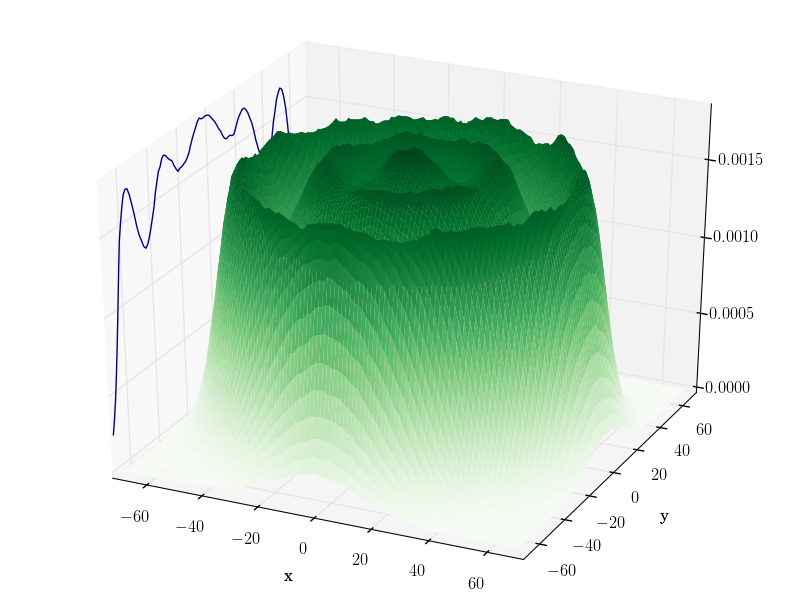
\includegraphics[scale=0.25]{../graphics/OBD/OBD_DMC/dist_out_QDots20c001_3D.png}}
  \subfigure{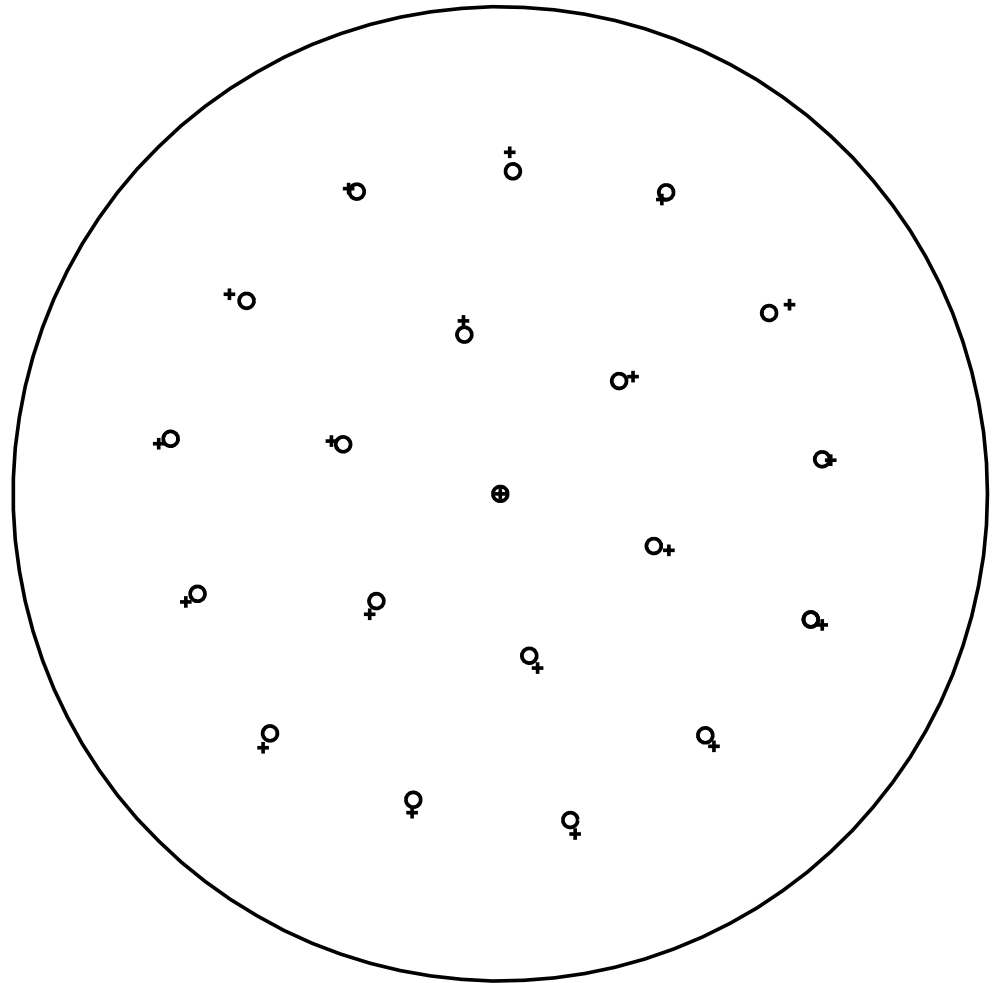
\includegraphics[scale=0.15]{../graphics/wigner/wigner20.png}}
  \label{fig:wigner20}
  \caption{OBD for a 20-particle two-dimensional quantum dot compared to the classical theoretical configuration taken from P. Galatola et al.~\textit{Eur. Phys. J. B} \textbf{50}, 549 (2006).}
 \end{center}
\end{figure}
\end{frame}

\begin{frame}
 This effect is called \textit{Wigner Crystallization} and is expected for low density electron gases when the \textbf{kinetic energy on average becomes far lower than the corresponding total potential energy}.
 \shift
 
 The connection between potential and kinetic energy is given by the \textit{virial theorem}
 
 \begin{equation}
  V(\mathbf{r}) \propto r^\gamma \quad\longrightarrow\quad \langle \OP{T} \rangle = \frac{\gamma}{2} \langle \OP{V} \rangle, \label{eq:virial}
 \end{equation}
 \shift
 
 Systems with similar proportionality constant follow the same effective potential, that is, they have similar eigenstates.

\end{frame}

\begin{frame}
 \captionsetup[subfloat]{labelformat=empty}
\begin{figure}[h]
 \begin{center}
  \subfigure[$N=6$]{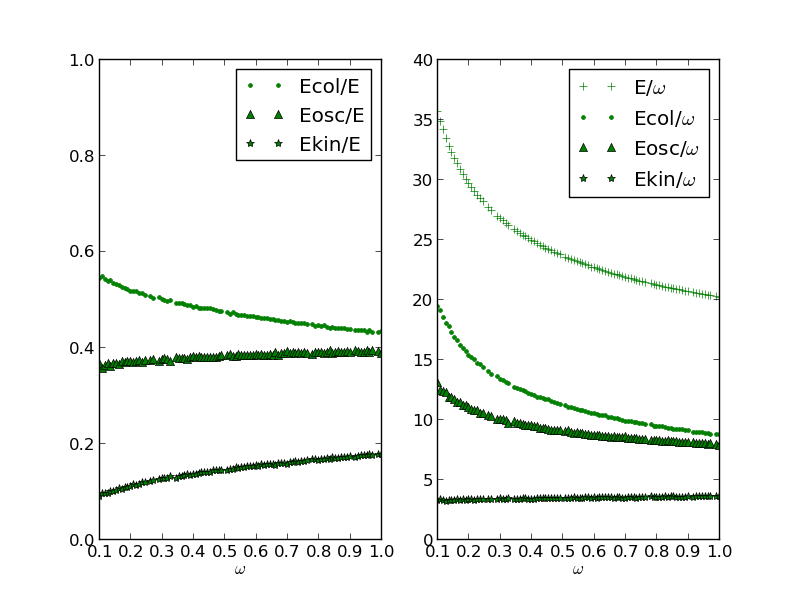
\includegraphics[scale=0.25]{../graphics/VirialPlots/E_vs_w_E6.png}}
  \subfigure[$N=42$]{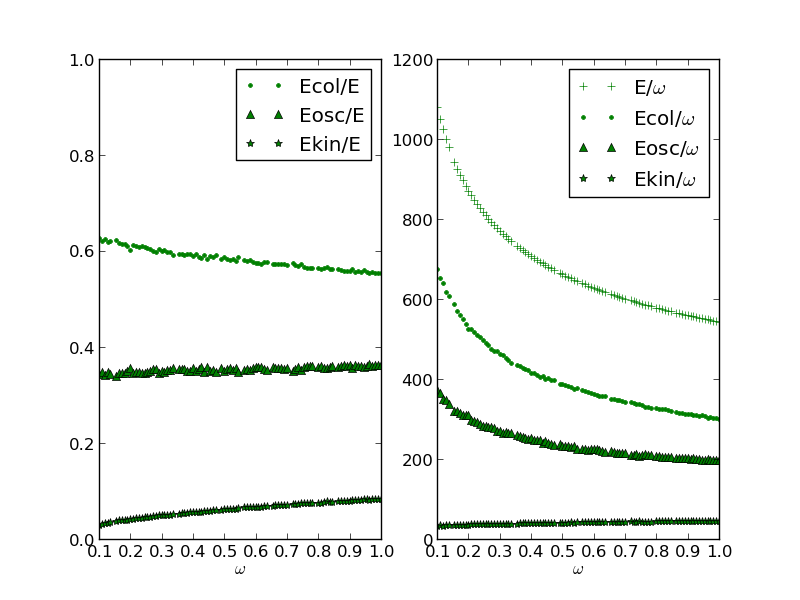
\includegraphics[scale=0.25]{../graphics/VirialPlots/E_vs_w_E42.png}} \\
  \caption{The relative magnitude of the expectation value of the different energy sources as a function of the frequency $\omega$ (left) together with the magnitude of the sources' energy contributions scaled with the oscillator frequency (right).}
  \label{fig:E_dist_qdots}
 \end{center}
\end{figure}
\end{frame}

% 
% \begin{frame}
%  Conclusions:
%  \shift
%  The kinetic energy falls whereas the total potential energy increases.
%  \shift
%  The kinetic energy is proportional to the frequency
%  
%  \begin{equation}
%   \langle \OP{T} \rangle \propto \omega.
%  \end{equation}
%  
% \end{frame}

\begin{frame}
 \frametitle{Transition into a Wigner crystal?} 
 \captionsetup[subfloat]{labelformat=empty}
 \begin{figure}[h]
 \begin{center}
  \subfigure[$N=6$]{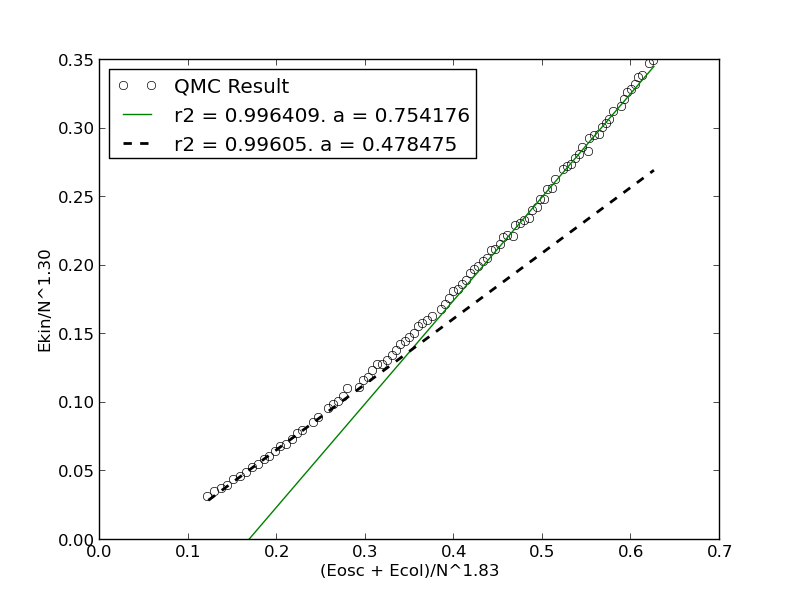
\includegraphics[scale=0.3]{../graphics/VirialPlots/E_vs_w_V6.png}}
  \subfigure[$N=42$]{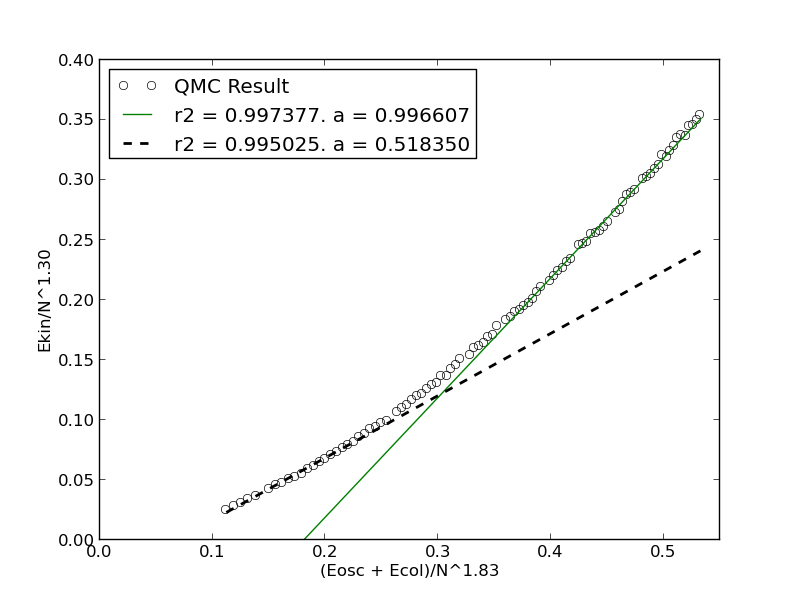
\includegraphics[scale=0.3]{../graphics/VirialPlots/E_vs_w_V42.png}} \\
  \caption{The total kinetic energy vs. the total potential energy of two dimensional quantum dots. NB: Collapsed.}
  \label{fig:V_dist_qdots}
 \end{center}
\end{figure}
\captionsetup[subfloat]{labelformat=parens}
\end{frame}

\begin{frame}
 \frametitle{Preliminary double-well density}
 
 \begin{figure}[h]
 \begin{center}
 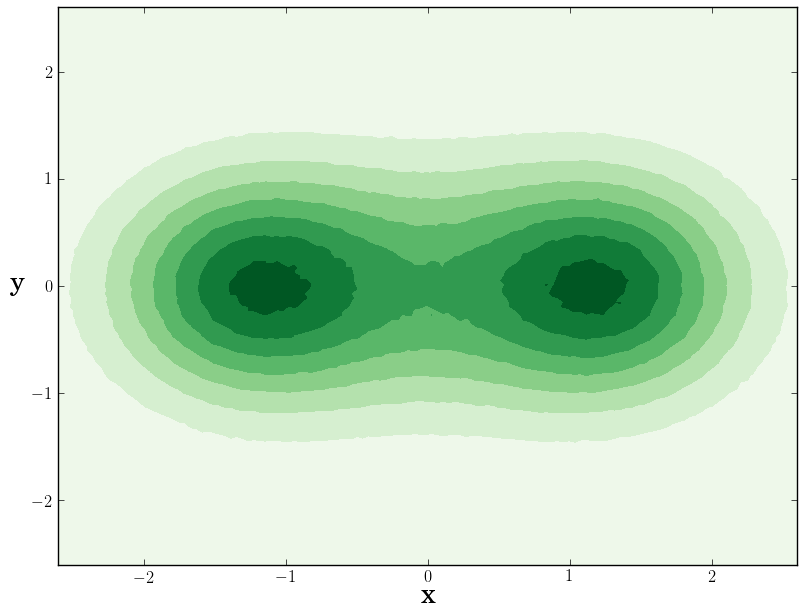
\includegraphics[scale=0.25]{../graphics/DoubleWell.png}
  \caption{A countour plot of the trial wave function for a two-particle double-well quantum dot with the wells separated at a distance $R = 2$.}
  \label{fig:doubleWell}
 \end{center}
\end{figure}
 
\end{frame}


\subsection{Atomic systems}

\footnotesize
\begin{frame}
\frametitle{Atoms}
 \begin{table}
\begin{center}
\begin{tabular}{lp{1cm}ccl}
Atom (N) & & $E_\mathrm{VMC}$ & \qquad $E_\mathrm{DMC}$ & \qquad\,\, Expt. \\
\hline\hline
\ \\
He (2) & \qquad & -2.8903(2) & \qquad -2.9036(2) & \qquad $-2.9037$ \\
\ \\
% Be & \qquad & -14.145(2) & \qquad -14.657(2)  & \qquad $-14.6674$\\
% \ \\
% Ne & \qquad & -127.853(2) & \qquad -128.765(4) & \qquad $-128.9383$  \\
% \ \\
% Mg & \qquad & -197.269(3) & \qquad -199.904(8) & \qquad $-200.054$  \\
% \ \\
% Ar & \qquad & -524.16(7) & \qquad -527.30(4) & \qquad $-527.544$   \\
% \ \\
Kr (36) & \qquad & -2700(5) & \qquad -2749.9(2) & \qquad $-2752.054976$  \\
\ \\
\end{tabular}
\caption{Ground state energies for atoms calculated using Variational - and Diffusion Monte-Carlo.}
\label{tab:AtomsRes}
\end{center}
\end{table}
\normalsize
\end{frame}

% \begin{frame}
%  Quantum dots results for VMC and DMC were significantly more similar. 
%  \shift
%  Worse for the non-noble gases and for higher number of particles.
%  \shift
%  Easier to excite an electron into the next sub-shell (next $l$) than to the next $n$.
%  \shift
%  The hydrogenic ansatz only accounts for \textit{bound states}. 
% \end{frame}

\begin{frame}
\frametitle{Densities: The noble gases}
 \begin{figure}
 \begin{center}
   \subfigure{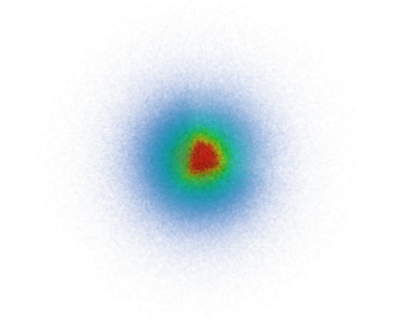
\includegraphics[scale=0.3]{../graphics/OBD/OBD_Atoms/3D/Helium.png}} 
%    \subfigure{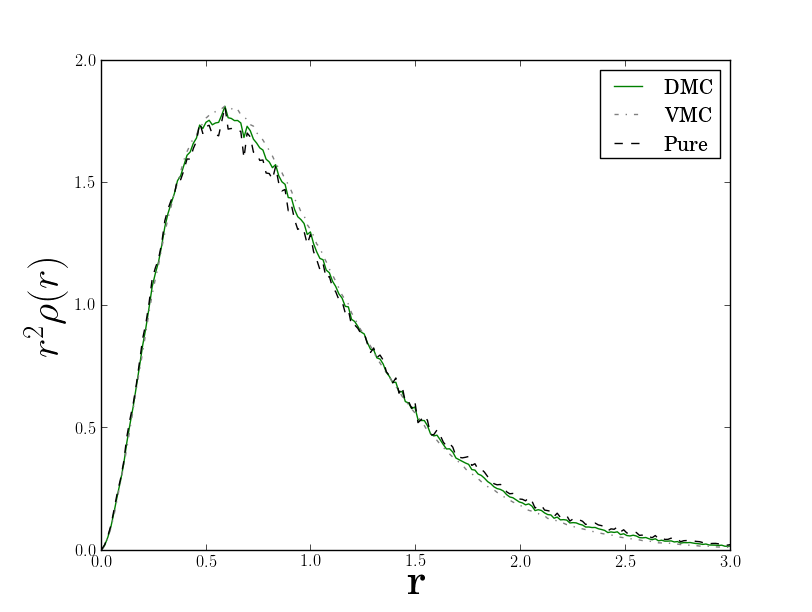
\includegraphics[scale=0.15]{../graphics/OBD/OBD_Atoms/2D/Helium.png}}  \\
   \subfigure{\includegraphics[scale=0.3]{../graphics/OBD/OBD_Atoms/3D/Neon.png}} 
%    \subfigure{\includegraphics[scale=0.15]{../graphics/OBD/OBD_Atoms/2D/Neon.png}}  \\
%    \subfigure{\includegraphics[scale=0.4]{../graphics/OBD/OBD_Atoms/3D/Argon.png}} 
%    \subfigure{\includegraphics[scale=0.3]{../graphics/OBD/OBD_Atoms/2D/Argon.png}}  \\
%    \subfigure{\includegraphics[scale=0.2]{../graphics/OBD/OBD_Atoms/3D/Krypton.png}} 
%    \subfigure{\includegraphics[scale=0.15]{../graphics/OBD/OBD_Atoms/2D/Krypton.png}}  \\
  \caption{One-body densities for helium and neon. }
  \label{fig:OBD_noble_Atoms_2D_combo}
 \end{center}
\end{figure}
\end{frame}



\begin{frame}
\frametitle{Densities: The alkaline earth metals}
  \begin{figure}
 \begin{center}
   \subfigure{\includegraphics[scale=0.3]{../graphics/OBD/OBD_Atoms/3D/Beryllium.png}} 
%    \subfigure{\includegraphics[scale=0.15]{../graphics/OBD/OBD_Atoms/2D/Beryllium.png}}  \\
   \subfigure{\includegraphics[scale=0.3]{../graphics/OBD/OBD_Atoms/3D/Magnesium.png}} 
%    \subfigure{\includegraphics[scale=0.15]{../graphics/OBD/OBD_Atoms/2D/Magnesium.png}}  \\
  \caption{Three dimensional one-body density for alkaline earth metals; beryllium  and magnesium.}
  \label{fig:OBD_alkaline_Atoms_2D_combo}
 \end{center}
\end{figure}
\end{frame}

\begin{frame}
\frametitle{Molecules}
 \begin{table}
\begin{center}
\begin{tabular}{lcccrlrr}
Molecule (N) & $R$ & & \qquad & $E_\mathrm{VMC}$ & & \qquad $E_\mathrm{DMC}$ & \qquad\,\, Expt.\\
\hline\hline
\ \\
$\mathrm{H_2}$ (2) & 1.4   & &\qquad & -1.1551(3)    & \qquad   & -1.1745(3)   & \qquad $-1.1746$     \\
\ \\
% $\mathrm{Li_2}$& 5.051 & &\qquad & -14.743(3)    & \qquad   & -14.988(2)   & \qquad $-14.99544$     \\
% \ \\
% $\mathrm{Be_2}$& 4.63  & &\qquad & -28.666(5)    & \qquad   & -29.301(5)   & \qquad $-29.33854(5)$  \\
% \ \\
% $\mathrm{B_2}$ & 3.005 & &\qquad & -47.746(7)    & \qquad   & -49.155(5)   & \qquad $-49.4184$    \\
% \ \\
% $\mathrm{C_2}$ & 2.3481& &\qquad & -72.590(8)    & \qquad   & -74.95(1)    & \qquad $-75.923(5)$   \\
% \ \\
% $\mathrm{N_2}$ & 2.068 & &\qquad & -102.78(1)    & \qquad   & -106.05(2)   & \qquad $-109.5423$    \\
% \ \\
$\mathrm{O_2}$ (16) & 2.282 & &\qquad & -143.97(2)    & \qquad   & -148.53(2)   & \qquad $-150.3268$    \\
\ \\
\end{tabular}
\caption{Ground state energies for homonuclear diatomic molecules calculated using VMC and DMC. }
\label{tab:MoleculesRes}
\end{center}
\end{table}
\end{frame}


\begin{frame}
 \begin{figure}[h]
 \begin{center}
   \subfigure{\includegraphics[scale=0.2]{../graphics/OBD/OBD_MOL/Li2_3D.png}} 
   \subfigure{\includegraphics[scale=0.15]{../graphics/OBD/OBD_MOL/Li2_2D.png}}  \\
   \subfigure{\includegraphics[scale=0.2]{../graphics/OBD/OBD_MOL/O2_3D.png}} 
   \subfigure{\includegraphics[scale=0.15]{../graphics/OBD/OBD_MOL/O2_2D.png}}
  \caption{One-body densities of $\mathrm{Li_2}$ (top) and $\mathrm{O_2}$ (bottom). }
  \label{fig:OBD_Molecules}
 \end{center}
\end{figure}
\end{frame}

% \begin{frame}
%  \frametitle{Parameterizing Force-field Potentials}
% 
% The potential energy in a molecular dynamics simulation is \emph{any energy source which can be used to alter the kinetic energy of the atoms}.
% \shift
% 
% The electrons are not simulated, hence the \emph{total energy of the quantum mechanical system correspond to the molecular potential}.
% 
% \begin{equation}
%  F_\mathrm{MD}(R) = \frac{\mathrm{d} V_\mathrm{MD}}{\mathrm{d} R} = \frac{\mathrm{d} E}{\mathrm{d} R}.
% \end{equation}
% \shift
% 
% This energy vs. $R$ relation can be parameterized using Quantum Monte-Carlo.
% 
% 
% \end{frame}

\begin{frame}
\frametitle{Parameterizing force-field potentials}
 \begin{figure}
 \begin{center}
  \includegraphics[scale=0.5]{../graphics/R_VS_E/LD.png}
  \caption{The Lennard-Jones 12-6 potential.}
  \label{fig:LennardJones}
   \end{center}
\end{figure}
\end{frame}

\begin{frame}
\frametitle{Parameterizing force-field potentials}
 \captionsetup[subfloat]{labelformat=empty}
 \begin{figure}
 \begin{center}
  \subfigure[$\mathrm{H_2}$]{\includegraphics[scale=0.25]{../graphics/R_VS_E/R_vs_E_hyd_pure.png}}
  \subfigure[$\mathrm{Li_2}$]{\includegraphics[scale=0.25]{../graphics/R_VS_E/R_vs_E_lit_pure.png}} 
  \caption{The distance between the atoms $R$ vs. the potential and total energy calculated using QMC.}
  \label{fig:molecules_R_vs_E}
 \end{center}
\end{figure}
\end{frame}



 













